The efficient scheduling problem has been intensively studied for asymmetric systems.
In this section we describe four scheduling approaches that target such systems.
The first three are based on separating the tasks into groups of critical and non-critical tasks and assign each group to one core type: the critical tasks to the fast cores and the non-critical tasks to the slow cores.
The difference between these three approaches is the way of considering a task critical.
First is the Criticality-Aware scheduler (CATS)\cite{Chronaki:ICS2015}, which detects the critical tasks based on their \textit{bottom level}.
Secondly, the Critical Path scheduler (CPATH), proposed in this paper, that detects the critical path of the dynamic (TDG) with the help of \textit{bottom cost} based priorities.
The Hybrid Criticality scheduler (HYBRID), proposed in this paper, uses both bottom level and bottom cost based priorities.
Last, we describe a dynamic implementation of HEFT scheduler (dHEFT)~\cite{HEFT}, that for every task it detects the processor that finishes its execution at the earliest possible time.
All of the described schedulers operate at runtime on the dynamic snapshots of the TDG. 
CPATH, HYBRID and dHEFT perform on-line profiling of the task execution time without considering inter-task communication costs, given the uncertainty of data movement latency that hides in the cache hierarchy of an asymmetric multi-core system with prefetching. 
%but none of these schedulers track the inter-task communication costs.


\lstset{basicstyle=\footnotesize\ttfamily,
        emphstyle=\bfseries,
        columns=fixed,
        numbers=none,
        moredelim=*[l][\textit]{//},
        moredelim=*[l][\bfseries]{\#},
        literate={...}{\dots}3
} 
\subsection{Criticality-Aware Task Scheduler}
\label{sec.cats}
The Criticality-Aware Task Scheduling generally applies to task-based programming models supporting task dependencies, but for simplicity we explain it in the context of the OmpSs programming model.
CATS uses bottom-level longest-path priorities and consists of three steps:
%\begin{itemize}

\textbf{Task prioritization}: when a task is created and added to the TDG, it is assigned a priority and the priority of the rest of tasks in the graph is updated accordingly.
 %Since the task graph is generated at runtime, there is no way to statically compute the priority that will be given to a task. 

\textbf{Task submission}: when a task becomes \textit{ready}, i.e., all its predecessors finished their execution, it is submitted to a \textit{ready queue}. At this point, the algorithm decides whether the task is considered \textit{critical} or \textit{non critical}. The task is then inserted in the corresponding ready queue: tasks in the \textit{critical ready queue} will be executed by fast cores, and tasks in the \textit{non-critical ready queue} will be executed by slow cores.

\textbf{Task-to-core assignment}: when a core becomes idle, it tries to retrieve a task from its corresponding ready queue to execute it. If the queue is empty, it might try to steal from the other queue according on the work stealing policy. %Currently, we support two work stealing mechanisms: \textit{simple} work stealing, i.e., fast cores can steal from slow cores; and \textit{bidirectional} (\textit{2DS}) work stealing, i.e., both types can steal from the other. The default policy is \textit{simple}.
%\end{itemize}

These steps are performed dynamically and potentially in parallel in different cores. Thus, while some tasks are being prioritized, previously created tasks may be submitted, and others assigned to available cores or executed.

To give an overview of the scheduling process, Figure~\ref{botlevels} shows a scheme of the operation of CATS. In the TDG on the left, each node represents a task and each edge of the graph represents a dependency between two tasks. The number inside each node is the \textit{bottom level} of the task: the length of the longest path in the dependency chains from this node to a leaf node. The priority of a task is given by its bottom level. The pattern-filled nodes indicate tasks that are considered critical. The number outside each node is the task id and is used in the text to refer to each task. Critical tasks are inserted in the critical queue, and non-critical tasks to the non-critical queue. The insertion is ordered with the highest priorities at the head of the queue and the lowest priorities at the tail. Slow cores retrieve tasks from the head of the non-critical queue and fast cores from the critical queue. The following sections describe these scheduling steps in~detail.


\begin{figure}[t]
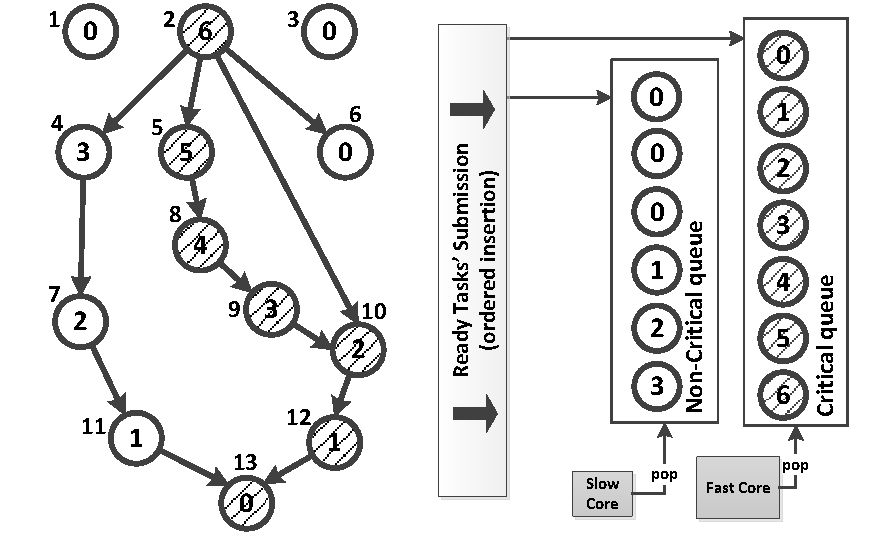
\includegraphics[width=\columnwidth]{images/fig_1.pdf} 
\centering
\caption{Task submission with CATS. Nodes are marked with the \textit{bottom level} of each task. Pattern-filled nodes mark the critical tasks.}
\label{botlevels}
\vspace{-0.5cm}
\end{figure}


\subsubsection{Task Prioritization}

Each task in the TDG has a list to include its predecessors (\textit{plist}). Every time an edge is added into the TDG on the creation of a new task, the corresponding predecessor of the dependency is added in the \textit{plist} of its successor. For example, in Figure~\ref{botlevels}, when the dependency between tasks~2 and~5 occurs, the task number~2 is inserted into the \textit{plist} of the task number~5. Thus, the \textit{plist} of task number~5 becomes $\{$2$\}$. Accordingly, the \textit{plist} of task number~10 will be $\{$2, 9$\}$ when the edge~9$\rightarrow$10 is inserted to the TDG. 

%Right after the occurrence of a dependency between two tasks, the task prioritization step takes place, once for each edge of the graph. 
%represented by the edges in the graph, that connect one predecessor task with one successor task.

The priority given to a task is the \textit{bottom level} of the task. The \textit{bottom level} is computed by traversing the TDG upwards starting from the successor that the currently created edge is pointing to. The priority of this successor is 0 because it is a leaf node of the graph, as it is the last created task. Then, using \textit{plist} for each task, the algorithm navigates to the upper levels of the TDG and updates the priority on each visited node. This way not all the graph is updated, but only the tasks that are predecessors in the paths to the new edge. The algorithm also stops going up through a path, when it finds a priority larger than the one it would be updated to.

Listing~\ref{creation} shows the algorithm for task prioritization. The complexity of this is \textit{O($n^2$)}, \textit{$n$} being the number of tasks. This function is called on the creation of a new edge with the successor as argument. The algorithm traverses the \textit{plist} of the successor task (line 5) and if the priority of the current predecessor is lower than the bottom level of the successor plus one, it updates the current predecessor's priority to that value (lines 7-8). If the updated predecessor task is ready (i.e., it sits in one of the ready queues), the scheduler reorders the ready queue so it remains ordered considering the updated priority (lines 9-10). Then, the same actions are performed recursively for each predecessor of the \textit{plist} to update all the possible upward paths from the successor. 

The terminate conditions for the TDG navigation are two: \textit{(a)} if the \textit{plist} of the current task (\texttt{currPred}) is empty, so either we reach an entry node or the predecessors of the task have finished execution; or \textit{(b)} if the priority of the current task (\texttt{currPred}) remains unchanged, which means that the successor task (\texttt{succ}) does not belong to the longest path because its predecessor already has a higher priority. 
\begin{lstlisting}[float, emph={void,if,return,non_critical_queue, critical_queue,prioritize_task}, captionpos=b, caption={Pseudo-code task prioritization with CATS.},label=creation, emph={[2]mat}, emphstyle={[2]}, aboveskip={0\baselineskip}, frame=tb, belowskip={-0.4cm}]
1 void prioritize_task(task *succ) {
2  int blev = succ->priority;
3  list plist = plistOf(succ);
4  task *currPred;
5  while( not isEmpty(plist) ) {
6    currPred = plist.next();  
7    if(priorityOf(currPred) < blev+1) {
8     currPred->priority = blev+1;
9     if(isReady(currPred)) 
10     readyQueueOf(currPred)->reorder();
11    prioritize_task(currPred);
12   }
13 }
14}
\end{lstlisting}
\subsubsection{Task Submission}

%CATS supports two task submission policies: the \textit{flexible} policy adds more task in the critical queue for the fast cores, while the \textit{strict} policy reduces the number of critical tasks.

The purpose of this step is to divide the tasks into two groups: \textit{critical} and \textit{non-critical}. Critical tasks are tasks that belong to the longest path of the dynamic TDG, namely the path  with the maximum number of tasks (or nodes). Thus, the longest path starts from the task with the maximum bottom level. At runtime, the longest path changes as tasks complete execution and new tasks are created. CATS manages to detect these changes and dynamically decide if the submitted task belongs to the longest path of the TDG.

When a task's dependencies are satisfied, the task becomes ready for execution and is to be inserted in the \textit{ready queues}. Ready queues are priority queues that keep tasks in a decreasing order of task priorities, i.e., the task with the maximum priority resides on the head of the queue. Critical tasks are inserted in the critical queue and non-critical tasks in the non-critical queue. The pattern-filled nodes in Figure~\ref{botlevels} represent the critical tasks in that graph. 

%This way, tasks in the critical queue will then be scheduled to fast cores, and non-critical tasks to slow cores.

%By keeping track of the last discovered critical task%task with the maximum priority
To determine the criticality of a task, CATS keeps track of the last discovered critical task. Then, for each task that becomes ready, CATS checks the following conditions:
%, our approach to detect critical tasks in the graph is to check the following two conditions for each task that becomes ready:
\textit{(a)} if the priority of the current ready task is higher or equal to the priority of the last discovered critical task and, \textit{(b)} if the current ready task is the highest-priority immediate successor of the last discovered critical task.

%%%%%%%%%%%%%%%%%%%%%%%%%%%%%%%%%%%%%%%%
\if 0 %flexible strict explanation
In the first case, the algorithm detects new longest paths that may have been created by the application throughout the execution of a prior longest path. In this case, the scheduler can either be \textit{strict} or \textit{flexible}:
\begin{itemize}
 \item{\textit{Strict}: marks as critical tasks with priority higher than the priority of the last critical task.}
 \item{\textit{Flexible}: marks as critical tasks with priority higher or equal to the priority of the last critical task.} 
 \end{itemize}
As a result, the flexible scheduler ends up with more critical tasks than the strict. The flexibility of the scheduler can be set by the programmer through an environment variable.
\fi % about flexible/strict explanation
%%%%%%%%%%%%%%%%%%%%%%%%%%%%%%%%%%%%%%%%%%%%
\begin{figure}[tl!]
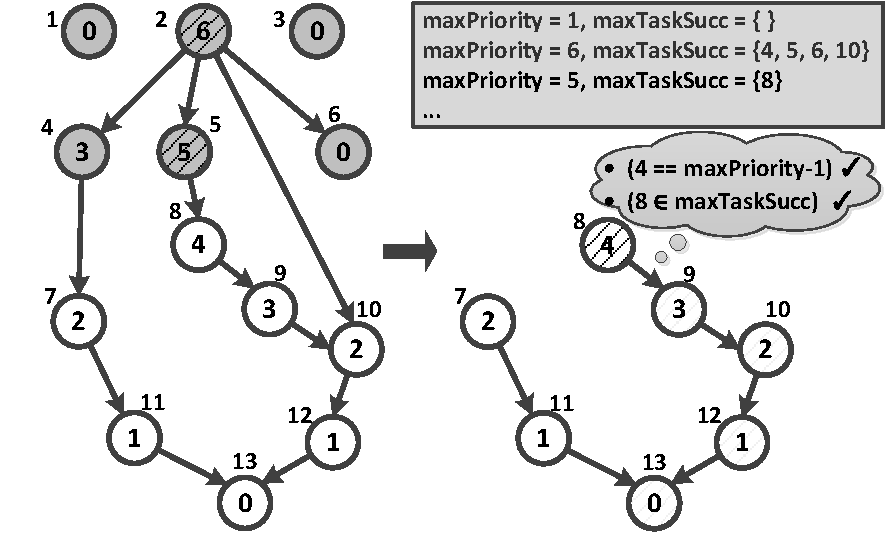
\includegraphics[width=\columnwidth]{images/fig_2.pdf} 
\centering
\caption{Task submission. Gray nodes indicate finished tasks and pattern-filled nodes indicate critical tasks.}
\label{submitFig}
\vspace{-0.5cm}
\end{figure}
The task that satisfies the second condition is a task with a lower priority than the maximum but the task belongs to the longest path because it is the highest priority immediate successor of the last detected critical task. 

Listing~\ref{submission} shows a simplified version of the task submission code, that is of complexity \textit{O($n$)} (\textit{$n$} is the number of tasks). The variable \texttt{maxPriority} (line 1) is used to store the priority of the last critical task, and \texttt{maxPriorityTask} (line 2) is used to store the last critical task. Initially, \texttt{maxPriority} is set to 1 and \texttt{maxPriorityTask} is set to \texttt{NULL}. This avoids the scheduling of independent tasks (i.e., tasks with zero priority) to fast processors at the start of the execution. On the first ready task, if its priority is higher or equal than 1 (line 5) , it is considered to be the first task of the longest path. Therefore, it is inserted in the critical queue and the variables \texttt{maxPriority} and \texttt{maxPriorityTask} are updated accordingly (lines 9-11) to determine correctly the criticality of the next submitted task.

If the priority of the submitted task is equal to \texttt{maxPriority - 1}, we check if it also belongs to the successors of the task with the maximum priority (lines 6-7) and therefore to the longest path. If these two conditions are met, the task is determined to be critical, it is inserted in the critical queue and, as before, the variables \texttt{maxPriority} and \texttt{maxPriorityTask} are updated (lines 9-11). In the rest of the cases the task is not considered critical and it is inserted in the non-critical queue.

Figure~\ref{submitFig} shows an example of a TDG during task submission. The gray nodes in the graph are tasks that have finished execution and the pattern-filled nodes are critical tasks. The numbers inside the nodes indicate their priority and the numbers outside the nodes show the task id, which is assigned in task creation order. The variable \texttt{maxPriority} corresponds to the priority of the last critical task and the \texttt{maxTaskSucc} is the list of the successors of the last critical task, filled with the task ids of the successors. Initially, \texttt{maxPriority} is set to~1 and \texttt{maxTaskSucc} is empty. When task~2 is about to be submitted, it is inserted in the critical queue because its priority is higher than the maximum, which at the beginning is~1. Then, the value of \texttt{maxPriority} is set to~6 (priority of task~2), and the \texttt{maxTaskSucc} list is updated with the successors of task~2. At the point where all the gray tasks have finished execution, the values of \texttt{maxPriority} and \texttt{maxTaskSucc} are updated as shown  in Figure~\ref{submitFig}. For every newly-ready task, the conditions listed above are evaluated. When task~7 is submitted, it is not considered as critical because it does not belong to the \texttt{maxTaskSucc} list and its priority is not equal to \texttt{maxPriority-1}. Contrarily, task 8 satisfies both conditions and so the task is inserted in the critical queue.

\begin{lstlisting}[float, emph={void,if,return,non_critical_queue, critical_queue,submit_task}, captionpos=b, caption={Pseudo-code for task submission with CATS.},label=submission, emph={[2]mat}, emphstyle={[2]}, aboveskip={0\baselineskip}, frame=tb, belowskip={-0.4cm}]
1 int maxPriority = 1;
2 task *maxPriorityTask = NULL;
3
4 void submit_task(task *t) {
5  if( t->priority >= maxPriority or
6     (t->priority == maxPriority-1 and
7      t $\in$ succListOf(maxPriorityTask)) )
8  { //the task is critical
9    critical_queue.push(t);
10   maxPriority = priorityOf(t);
11   maxPriorityTask = t;
12   return;
13 }
14 //the task is non-critical
15 non_critical_queue.push(t);     
16}
\end{lstlisting}

\subsubsection{Task-to-Core Assignment}
\label{sec.cats.assignment}
Task-to-core assignment takes place dynamically and in parallel to the previous steps and its time complexity is \textit{O($n$)}, \textit{$n$} being the number of tasks. When a core becomes idle, it checks the corresponding ready queue (depending on the core type) to get a task to execute. Fast cores retrieve critical tasks from the critical queue, while slow cores retrieve non-critical tasks from the non-critical queue. Each ready queue is shared among the cores of the same type so there is no need for work stealing among cores of the same type. 

If tasks in an application are imbalanced, i.e., the majority are non-critical and only a few tasks are critical, or vice versa, one of the types of processors would be overloaded and the other would starve for work. This can happen in applications with wide graphs and a large amount of tasks, where the ratio between critical tasks and the total amount of tasks may be small. To leverage the resources, the work-stealing mechanism for CATS lets fast cores steal work from slow cores whenever the critical queue becomes empty. 
%Also, CATS can be configured to perform \textit{bidirectional work stealing} so slow processors can also steal tasks from the critical queue if the non-critical queue is empty. 
%We evaluate these different options and show the results in the next section.

\section{Critical Path Scheduler}
\label{sec.scheduling.cpath}
\begin{figure}[tr]
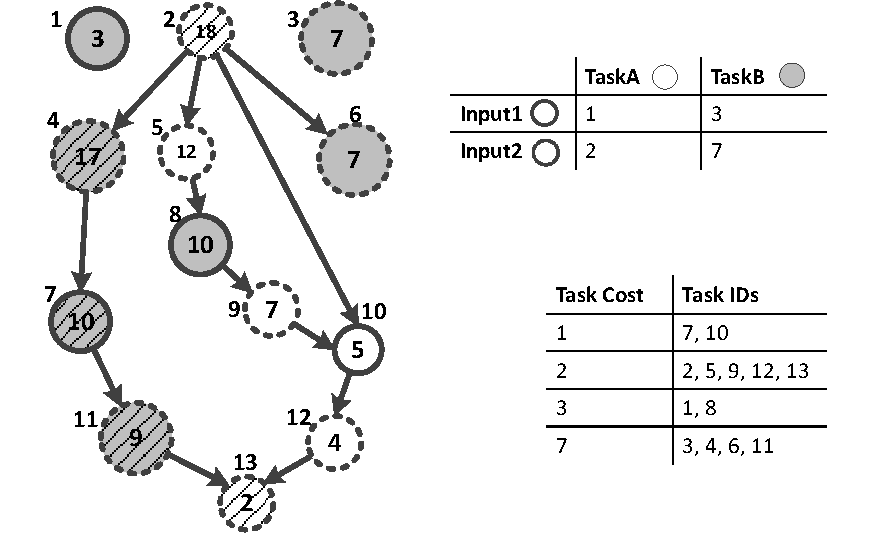
\includegraphics[width=\columnwidth]{images/cpath_priorities.pdf} 
\centering
\caption{Priority assignment taking into account the task costs. Task costs are assumed known and are shown in the tables.}
\label{cpath}
\vspace{-0.5cm}
\end{figure}


The Critical Path scheduler (CPATH) dynamically detects the critical path of the TDG.
Like CATS, CPATH separates tasks into two groups: critical and non-critical tasks.
The detected critical tasks are executed by the fast cores in the system and non-critical tasks are executed by slow cores.
The difference with CATS is the algorithm for critical path detection.
CPATH takes into account the task execution time, about which CATS is unaware.
To do so, CPATH implements a more complex and accurate critical path detection algorithm that takes into account task execution time.

CPATH scheduler consists of three steps:
%\begin{itemize}

\textbf{Task prioritization}: this step takes place when a task is finishing its execution. This is different than CATS since at the end of a task execution the algorithm may record the task execution time (task cost).
%might track a new (unknown) task cost. 
According to the discovered task cost CPATH assigns priorities to tasks by traversing the TDG from top to bottom, introducing the cost of \textit{O($2n^2$)}, where \textit{$n$} is the number of tasks.

\textbf{Task submission}: when a task becomes \textit{ready}, it is submitted to a \textit{ready queue}. At this point, CPATH decides whether or not the task is \textit{critical} and inserts it in the corresponding ready queue. This step has only slight implementation differences with CATS and complexity of \textit{O($n$)}.

\textbf{Task-to-core assignment}: this step is identical to CATS.
% and supports the same work stealing mechanisms.

%\end{itemize}

\subsection{Task Prioritization}
%explanation of the slist (successors' list)

Each task of the TDG keeps a list with its successors (\textit{slist}).
This list is being built when an edge (dependency between two tasks) is added in the TDG.
So when a task dependency occurs, the corresponding successor task is added in the \textit{slist} of its predecessor.
For example, on Figure~\ref{cpath}, when the dependency between tasks 2 and 4 occurs, the \textit{slist} of task number 2 becomes \{4\}. 
This goes on for all the added edges of the TDG, therefore when the edge~2$\rightarrow$5 is inserted in the TDG, the task number 5 is inserted in the \textit{slist} of task number 2; so the \textit{slist} of task number 2 becomes \{4, 5\}.

The goal of this step is to assign priorities based on the \textit{bottom cost} of the tasks of the TDG.
We define the \textit{bottom cost} of a node on a directed acyclic graph as the maximum estimated time in the dependency chains from this node to a leaf node.
So the main difference between the \textit{bottom level} and the \textit{bottom cost} is the consideration of the estimated time.

Figure~\ref{cpath} is used to describe the priority assignment with CPATH.
The specific TDG contains tasks of two different types and two different input sizes.
Node color shows the different task types and the outline of the circle (dashed or solid) shows the different input sizes.
The upper table in Figure~\ref{cpath} indicates the execution time of the tasks according to their type and input size.
The algorithm assumes that task instances of the same type with the same input size have the same (or very similar) execution time.
To track this information, CPATH discovers the cost of every possible task type-input size duple (tt-is duple) that appears on the TDG.
The numbers inside the nodes show the bottom cost-based priorities that CPATH assigns and the numbers outside the nodes show their task ID.


%This task type-input size duple is denoted as tt-is and the algorithm assumes that the task with the same tt-is have the same execution time.
%So the execution time of the tasks differs according to the task type-input size duple (\texttt{tt-is} duple).
%CPATH discovers the cost for all the tt-is pairs and prioritizes the tasks according to their \textit{bottom cost} as shown on Figure~\ref{cpath}.
%The bottom cost of a node is equal to the maximum estimated time in the dependency chains from this node to a leaf node.

The task prioritization step takes place every time a task finishes execution. 
CPATH uses a vector to store task costs and keeps one entry per tt-is.
Because CPATH needs to discover the unbiased critical path of the TDG, it uses one of the core types as reference to track the task costs.
%So at the beginning of the execution tasks are executed on one of the core types during this cost-learning phase.
In our experiments we chose to use as reference the fast cores since this way the learning phase (that is, the phase where CPATH discovers the task costs) becomes shorter.
To avoid wrong task cost prediction of future tasks, CPATH ignores the first execution of each tt-is because usually it takes more time. 
\begin{lstlisting}[float, emph={for,in,void,if,return,updatePriorities,non_critical_queue, critical_queue,submit_task}, captionpos=b, caption={Pseudo-code for taskExit, the function called by the cores used as reference for tracking the task costs},label=cpathExit, emph={[2]mat}, emphstyle={[2]}, aboveskip={0\baselineskip}, frame=tb, belowskip={-0.4cm}]
1 void taskExit (task* finished) {
2  if( stateOf(finished) == init ) {
3    finished->state = in_progress;
4    return;
5  }
6  if( stateOf(finished) == in_progress ) {
7    timesSet[finished] = finished->execTime;
8    finished->state = tracked;
9  }
10 task* succ;
11 for( succ in finished->successors ) 
12   if( numPredecessorsOf(succ) == 1 ) {
13     lock();
14     if( succ $\notin$ entryNodes ) 
15       entryNodes->push(succ);
16       unlock();
17   }
18 list<task>* updatedList = new list<task>();
19 for( node in entryNodes) 
20   updatePriorities(node, updatedList);
21 for( node in updatedList ) 
22    node->unsetUpdated();
23}
\end{lstlisting}

Listings \ref{cpathExit} and \ref{cpathUpdate} show how the critical path scheduler performs task prioritization.
Whenever a task finishes execution on one of the cores used as reference (here: fast cores) the runtime makes a call to the \texttt{taskExit} routine shown in Listing~\ref{cpathExit}.
At this point, the runtime is aware of the execution time of the finished task.
This function has the responsibility to update the known task costs and also perform the prioritization of the tasks on the TDG.
The prioritization is done by the \texttt{updatePriorities} function of Listing~\ref{cpathUpdate}. 
This function is responsible for TDG traversal.

The \texttt{taskExit} function in Listing~\ref{cpathExit} takes as an argument the task that has just finished. 
In order to keep track of whether the execution time of the tt-is has been discovered we implement a small finite state machine within this stage.
Every tt-is has three possible states. 
The initial state is the \texttt{init} state; this means that the specific tt-is has not yet been executed so its execution time is totally unknown.
When a tt-is is executed for the first time its state changes from \texttt{init} to 
\texttt{in$\_$progress}. 
This means that a task of this tt-is has been executed once, but CPATH ignores this cost because the first instance may not be representative due to cold start effects and one sample may not be enough history for prediction.
While the tt-is of a node is in \texttt{init} or \texttt{in$\_$progress} state its execution time is considered to be 1.
%we have to ignore this execution because usually it takes too long and is not representative.
After the second execution of a tt-is the state of it becomes \texttt{tracked} meaning that the execution time has been tracked and can be used for the computation of the priorities.
%If the node does not have a known execution cost tracked, we consider its execution time to be 1.

After the first checks of the tt-is state (lines 2-9 of Listing~\ref{cpathExit}) the algorithm traverses the \textit{slist} of the finished task and searches for the successors that become ready by the end of the execution of this task.
This is identified by the fact that the ready-to-be successors have one unique (remaining) predecessor (e.g. the just finished task).
These successors are inserted in the \texttt{entryNodes} list (lines 11-16 of Listing~\ref{cpathExit}).
For each one of the entry nodes the \texttt{updatePriorities} function is called (line 19 of Listing~\ref{cpathExit}); this performs a top to bottom traversal of the TDG and updates the priorities.

\begin{lstlisting}[float, emph={for,in,void,if,return,non_critical_queue, critical_queue,submit_task}, captionpos=b, caption={Pseudo-code for task prioritization with CPATH},label=cpathUpdate, emph={[2]mat}, emphstyle={[2]}, aboveskip={0\baselineskip}, frame=tb, belowskip={-0.5cm}]
1 int updatePriorities (task* currT, list* updated) {
2   if( currT == NULL )  return 0;
3   if( isVisited(currT) )  
4     return priorityOf(currT);
5   successors = currT->successors;
6   int maxSucc = -1;
7   bool succVisited = true;
8  
9   for(succ in successors) {
10    int succPriority;
11    //Avoid double update
12    if( !isUpdated(succ) || !isVisited(succ) ) {
13      succPriority = updatePriorities(succ, updated);
14      succ->setUpdated();
15      updated->push(succ);
16    }
17    else 
18      succPriority = priorityOf(succ);
19    if(succPriority > maxSucc)
20       maxSucc = succPriority;
21    succVisited = succVisited && isVisited(succ);   
22  }
23  if( timeIsTracked(currT) ) {
24    currT->priority = (maxSucc + timesSet[currT]);
25    if(succVisited && groupOf(currT) < twDetected) 
26      currT->setVisited();
27  }  
28  else
29    currT->priority = maxSucc + 1;
30    
31  return priorityOf(currT);  
32}
\end{lstlisting}

Due to the properties of the top-to-bottom TDG traversal, the algorithm has to make sure that every node is prioritized only once per \texttt{updatePriorities} call.
This is controlled by checking the \texttt{updated} flag of each node of the TDG.
To visualize this situation let us assume that task number 2 of the TDG on Figure~\ref{cpath} finishes.
Then the \texttt{entryNodes} list contains three tasks that will start the update: \{4, 5, 6\}.
The update that starts from task number 4 marks tasks 4, 7, 11 and 13 as updated.
Then, during the update of task number 5, the algorithm knows that task 13 has already been prioritized during the same update so there is no need to apply the algorithm at this node again.
This example does not show too much optimization because in this case the update of only one node is saved, but in real applications this node could have numerous successors for whom the priority update would be a large overhead.

The raising of the \texttt{updated} flag is something temporal and is only used for helping the prioritization of a single update.
There are cases when CPATH needs to raise a permanent flag in order to mark that the priority of the task will not change again in the future, e.g. it is the final priority.
This happens when the execution times of all the tt-is that appear on the TDG have been discovered, for the tasks that their priorities are up to date.
To mark these tasks CPATH uses the \texttt{visited} flag.
If a task is \texttt{visited}, there is no need to get prioritized again.
To clarify this, let us assume that in Figure~\ref{cpath} the task costs of the tt-is TaskA-Input2 and TaskB-Input2 are known.
During the next prioritization, tasks 11 (TaskB-Input2), 12 (TaskA-Input2) and 13 (TaskA-Input2) in the TDG will be set as visited, because their priorities consist of the sum of known task execution times and they do not have any successors (with unknown execution times).
So, an additional priority update in cases like this is redundant.
%So, the algorithm does not need to visit these nodes again on the current update, nor on a future priority update.


%Moreover, CPATH prioritization needs to make sure that the priority of a to-be-updated node is not the final priority.
%In case that the priority of a node is final then there is no need for updating this node.
%To perform this check, CPATH checks the \texttt{visited} flag of every node, which tells if the priority of the node is final.
%To understand what a final priority is, let's assume that CPATH has discovered the task costs of the tt-is TaskA-Input2 and TaskB-Input2 on the Figure~\ref{cpath}.
%This means that the tasks 11, 12 and 13 of the TDG are visited, because their priorities are not going to change since they consist of the sum of known task execution times and they don't have any successors.
%So, the algorithm does not need to visit these nodes again not on the current update, neither on a future priority update.



%For example, in Figure~\ref{cpath}


%Because one node might get updated more than once through different possible paths, we optimize the procedure by keeping the \texttt{updated} flag. 
%This flag tells whether the node has been updated during the prioritization that caused the exit of the same task. 
%This way duplicate updates on a single task exit are skipped and we make sure that the nodes are updated only once.
%At the end of this routine the updated flag is being unset because the nodes have to be updated in case a new task cost is discovered in a future task exit.

Listing~\ref{cpathUpdate} shows what happens during the the update of one entry node.
The arguments of this function are \texttt{currT}, that is the entry node being updated, and \texttt{updated}, that is the list with the updated nodes. 
This list is being filled throughout the priority update in order to unset the updated flag later.
The lines 2-4 of Listing~\ref{cpathUpdate} perform the checks that would cause the traversal to finish.
If the node is not visited, then the algorithm traverses its successors.
Note that, at this point, there is no check for updated flag, since tasks in the \texttt{entryNodes} are unlikely to be updated. 
Updated nodes can only be discovered through recursive calls and this check is performed later.
%this cannot happen from the entryNodes, only from recursive calls which is checked later.
If a successor is updated or visited, the priority update is skipped for the reasons explained above. 
Otherwise, the \texttt{updatePriorities} is called recursively for the current successor.
This happens until we detect a node that is updated, visited or is a leaf node (node with no successors) of the TDG.
When the algorithm reaches a node ready for update it calculates its priority by summing the highest priority of its successors to the execution time, if known, of the current node (lines 24, 29).
Finally, the visited flag of the task is being updated. 

There are three conditions that mark a task as visited: \textit{(a)} if its execution time is known (line 23),  \textit{(b)} if \textbf{all} of its successors are visited (line 25) or \textit{(c)} if we have encountered a taskwait (barrier) after the creation of this task (line 25).
%To mark a node as visited we have to check the following:
%\begin{itemize}
%\item If the execution time tracked of this tt-is is known (line 23)
%\item If \textbf{all} of the task's successors are visited (line 25)
%\item If we have encountered a taskwait (barrier) after the creation of this task (line 25)
%\end{itemize}
%In addition to the updated flag, the algorithm uses the \texttt{visited} flag.
%The algorithm is not using only the updated flag to mark the updates; each node in the TDG can be marked as \texttt{visited} as well.
%The \texttt{visited} flag tells to the algorithm that the node has a valid and unchangeable priority.
%This shows that the priorities of all the descendants of this task have valid execution times tracked and their priorities are computed according to these final values. 
%Thus there is no need to traverse the successors of a visited node and this is an important optimization of the algorithm.
%
%As described, the lines 2-4 of Listing~\ref{cpathUpdate} perform the checks that would cause the traversal to finish.
%If the node is not visited, then the algorithm traverses its successors.
%If a successor is updated or visited the update of priorities is skipped. 
%Otherwise, the \texttt{updatePriorities} is called recursively using the current successor as an entry node.
%This happens until we find a node that has been updated or is visited or a leaf node (node with no successors) of the TDG.
%When the algorithm reaches a node ready for update it calculates its priority by summing the highest priority of its successors with the execution time, if known, of the current node (lines 24, 29).
%If the node does not have a known execution cost tracked, we consider its execution time to be 1.
%Finally, the visited flag of the updated task is being updated. 
%To mark a node as visited we have to check the following:
%\begin{itemize}
%\item If the execution time tracked of this tt-is is valid
%\item If \textbf{all} of the task's successors are visited
%\item If we have encountered a taskwait after the creation of this task
%\end{itemize}
The last condition confirms that it is safe to mark this task as visited as there will be no future successors of this task on the current TDG. 
%The reason behind the last condition is that if we have encountered a taskwait \textbf{after} the creation of this task this means that there will be no future successors on the current TDG. 
%Thus, we do not need to worry about setting priorities on tasks that reside below the visited tasks of the TDG.
To track this information we use an atomic variable, \texttt{twDetected}, which is increased every time a taskwait is encountered.
At creation time, each task is assigned a group ID which is the value of the \texttt{twDetected} at that moment.
%This way the tasks are separated into groups according to the detected taskwaits.
%At creation time, tasks are separated into groups according to the detected taskwaits by assigning as group ID the value of the \texttt{twDetected} at that moment.
If the group ID of a task is less than the current \texttt{twDetected} value then this means that a taskwait has occurred after the creation of this task.

\subsection{Task Submission} 
The task submission is implemented using the same \texttt{critical} and \texttt{non-critical} ready queues as in CATS.
Listing~\ref{submission} can be used to describe the task submission of CPATH.
The only modification needed is in the condition of the lines 6 and 7 of Listing~\ref{submission}.
In addition to the \texttt{maxPriority}, CPATH keeps track of the \texttt{maxExecTime} which is the cost of the last discovered critical task.
CPATH extends the condition of the critical task consideration by checking whether the priority of the current task is equal to \texttt{maxPriority} - \texttt{1} or if it is equal to \texttt{maxPriority} - \texttt{maxExecTime}.
Moreover, the value of \texttt{maxExecTime} is updated accordingly to the \texttt{maxPriority}.

\subsection{Task-to-Core Assignment}
Task-to-core assignment in CPATH is identical to CATS as described in Section~\ref{sec.cats.assignment}. 
It takes place dynamically and in parallel to the previous steps.
Depending on the core type, whenever a core becomes idle it retrieves a task from its corresponding ready queue; fast cores are responsible for the execution of the tasks in the critical queue and slow cores for the tasks in the non-critical queue.
Each ready queue is shared among the cores of the same type so there is no need for work stealing among cores of the same type. 
Finally, as with CATS, the work-stealing mechanism prevents load imbalance by allowing big cores to steal work from the little cores.






\section{Hybrid Criticality Scheduler}
\label{sec.scheduling.hybrid}

The Hybrid Criticality Scheduler (HYBRID) is a combination of the CATS and CPATH scheduling policies.
HYBRID keeps the simplicity of the implementation of CATS and introduces the task execution time only if available.
This results in an efficient low-overhead scheduler that computes the critical path of a TDG more faithfully than CATS and with lower overheads than CPATH.
%The idea for this is again based on separating the critical and non-critical tasks and execute the critical tasks on the fast cores of the system.
This section describes HYBRID through its relation to CATS and CPATH described in Sections~\ref{sec.cats} and~\ref{sec.cpath}. 
We focus our description on the task prioritization, since task submission and task-to-core assignment for HYBRID are identical to CPATH.

As shown, CPATH computes priorities on task completion. 
The algorithm for priority computation is an expensive operation and is in the critical path of the execution:
on task completion the core becomes available but the start of the next task is delayed by priority computation.
Also, when multiple cores are completing tasks, there will be contention on accessing the TDG for priority computation.
On the other hand, CATS computes priorities during task creation.
The computation of priorities during task creation is more efficient because, unless there is nested parallelism, one core creates all tasks
and therefore there is no contention on priority computation. The downside is that there is potentially less information available 
on tt-is pair execution time on task creation, as some task type may have not been executed yet at the time all tasks are created.
%there is only one core involved in this procedure responsible for the creation of the tasks.
%In addition, the rest of the cores are exclusively used for executing tasks undisturbed.

%, where it is more unlikely to have information about the task execution time. 

%In an effort to reduce the scheduling overheads of CPATH, we implement HYBRID. 
HYBRID tracks task execution time on task completion and stores this information in a vector.
This means that it also implements the \texttt{taskExit} function of CPATH that is called on task completion but, in the case of HYBRID, \texttt{taskExit} is only responsible of recording the execution time of the exiting task.
This functionality is represented in lines 2-9 of Listing~\ref{cpathExit} and, after this code, the function returns.
% in HYBRID takes place during task creation because as described above this reduces the scheduling overheads.
The priority assignment, taking place on task creation, remains similar to CATS \footnote{All of the HYBRID scheduling steps have the same time complexity as CATS} with the only difference that task cost is used for priority computation only if known and, otherwise, the cost is assigned to 1 and priority is increased according to CATS (lines 7 and 8 of Listing~\ref{creation}).

%high-level differences:
%% This could be simplified, also given there is a short mention before
When comparing CPATH and HYBRID schedulers their logical operation is similar.
However the difference in their implementation may result in different task priorities potentially leading to different schedules.
For applications with small TDGs, HYBRID may not be able to compute an accurate critical path because task creation does not overlap with a sufficient amount of task exits.
%Therefore, priority computation will not have enough information about task execution time and HYBRID will prioritize based on bottom-level priorities (like CATS).
Therefore, task execution information will not be available during priority computation and HYBRID will prioritize based on bottom-level priorities (like CATS).
If the application has a large TDG and task creation overlaps with a sufficient amount of task exits, HYBRID will use bottom-cost priorities.
%CPATH on the other hand, updates priorities right after task cost is known, which leads to a more faithful critical path computation. 

\begin{figure}[tr]
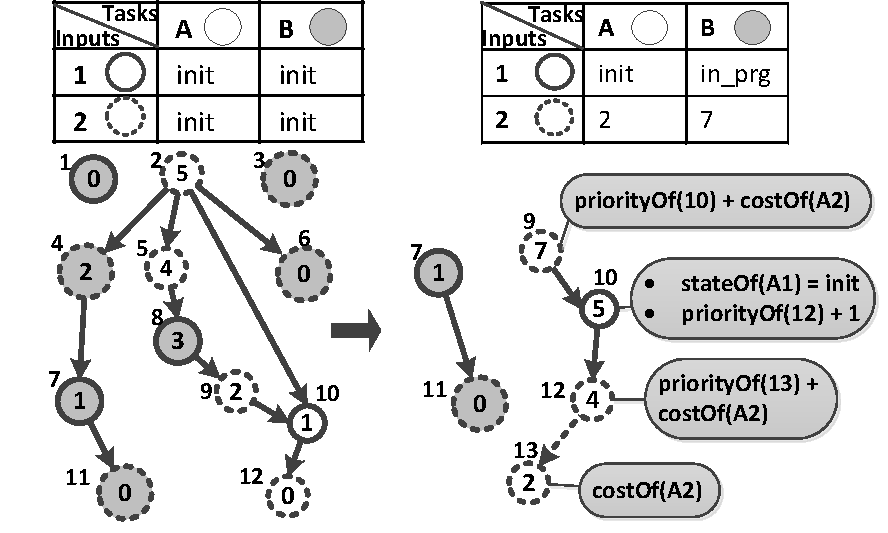
\includegraphics[width=\columnwidth]{images/hybrid_prioritization.pdf} 
\centering
\caption{Priority assignment with HYBRID scheduler. Priority update when the edge between tasks 12 and 13 is created}
\label{hybrid_priorities}
\vspace{-0.5cm}
\end{figure} 

Figure~\ref{hybrid_priorities} shows an example of task prioritization with HYBRID.
The tables show the state (or exec. time) of the tt-is pairs that appear on the TDG. Gray or white nodes indicate different task types (A or B respectively) and solid or dashed node outlines indicate task input size (1 or 2 respectively). The numbers inside the nodes show task priorities and the numbers outside the nodes show the task id.

On the leftmost TDG, the algorithm has no information about any of the tt-is costs.
As the leftmost table shows, for all the possible tt-is the state is \texttt{init} meaning no task has been executed yet.
Since the tasks of the TDG have been created, they have been prioritized using the CATS priority assignment method and the bottom level based priorities.
On the rightmost TDG, tasks 1, 2, 3, 4, 5, 6 and 8 have been executed and a new task has appeared on the TDG: task number 13.
When the edge 12$\rightarrow$13 is created, tasks begin to be prioritized.
Initially, the priority of the new task 13 is the cost of this task's tt-is, i.e., type A and input 2 (TaskA-Input2). 
Since there are no successors of this task, this becomes its initial priority.
Then, the \textit{plist} of task 13 is traversed and the priority of task 12 changes to priorityOf(13)+costOf(TaskA-Input2) since task 12 is corresponding to the TaskA-Input2 tt-is.
Moving to the upper levels, task 10 is of tt-is TaskA-Input1 that is on the \texttt{init} state, thus unknown cost.
This translates to the use of bottom level based prioritization so the priority of task 10 becomes priorityOf(12)+1.
Finally, task 9 is prioritized using the cost of the TaskA-Input2 tt-is and the TDG navigation stops since there are no other predecessors.

\if 0


Like CPATH, HYBRID prioritizes tasks according to their \textit{bottom cost} and/or their \textit{bottom level}.

HYBRID constitutes of three steps: \textit{Task Prioritization, Task Submission} and \textit{Task-to-core assignment.}


\subsubsection{Task prioritization}
The HYBRID scheduler prioritizes tasks according to their \textit{bottom cost} and/or their \textit{bottom level}.
The task prioritization step takes place during task creation.
%If when a dependency is created the execution time of the tt-is of the successor is known, then it is used for the prioritization.
If task cost information is available, HYBRID uses it to compute priorities.
Otherwise, the algorithm computes priorities the same way as CATS, that is, increasing the priority as we move to higher levels of the TDG.

%task execution time tracking:
As tasks are being executed HYBRID collects their execution times.
A vector is used to store the execution time of every tt-is discovered throughout the execution.
When a task finishes execution, HYBRID calls the \texttt{taskExit} function.
This function is responsible for tracking the execution time of the exiting task by storing it in the vector.
As in CPATH, \texttt{taskExit} ignores the first execution of every tt-is.
Therefore, the functionality of a small finite state machine is needed for each tt-is.
To start with, a tt-is is in the \texttt{init} state; when the tt-is has been executed once its state changes from \texttt{init} to \texttt{in$\_$progress} to skip the cost of the first execution.
After the second execution of the same tt-is, \texttt{taskExit} stores its execution time in the vector and its state becomes \texttt{tracked}.
This functionality is represented in the lines 2-9 of Listing~\ref{cpathExit}.
After this code, the function returns, since HYBRID does not perform any prioritization when a task is finishing execution.

The task prioritization step takes place when a new task is added to the TDG.
%Because the addition of a new task on the TDG always takes place at the (one) bottom of the graph, the use of the \textit{plist} (list of predecessors) of the tasks, is essential in order to perform a bottom-to-top TDG traversal.
HYBRID uses the \textit{plist} (list of predecessors as used in CATS) of the new task to navigate to the upper levels of the TDG and update the task priorities.

Listing~\ref{creation} shows the algorithm of the task prioritization with CATS.
Because HYBRID uses a very similar algorithm we will describe it using the same code while highlighting the differences.
When a new task is created, if its tt-is execution time is known, it is assigned as the priority of the new task. 
If there is no cost information the priority assigned to the new task is initially zero.
The \texttt{prioritize$\_$task} function is called on the creation of a new edge on the TDG between two tasks: the predecessor task and successor task.
It takes as argument the successor task and starts by traversing its \textit{plist} (line 5).
The HYBRID algorithm then checks whether the predecessor task has a tracked execution cost.
If so, it checks whether the priority of the current predecessor is lower than the priority of the successor plus the cost of the predecessor and, if this condition is met, the priority of the predecessor is updated accordingly.
In the case that the cost of the predecessor has not been tracked, the algorithm checks if the priority of the current predecessor is lower than the priority of the successor plus one (as on line 7 of Listing~\ref{creation}).
In the first case, HYBRID scheduler uses bottom cost based priorities, like CPATH, while in the latter case, it uses bottom level based priorities, like CATS.
In both cases, if the priority of the predecessor has changed and the predecessor task is a ready task (i.e. it sits on one of the ready queues) the corresponding ready queue is being reordered considering the updated priority (lines 9-10).

The same actions are performed for the predecessors of the upper levels of the TDG.
The algorithm, similarly to CATS, terminates if it encounters an empty \textit{plist} or if the priority of the current predecessor task (\texttt{currPred}) remains unchanged.


Figure~\ref{hybrid_priorities} shows an example of task prioritization with HYBRID.
The tables show the state (or the exec. time) of the tt-is pairs that appear on the TDG.
Gray or white nodes indicate different task types (type A or B respectively) and solid or dashed node outlines indicate the task input size (input 1 or 2 respectively).
The numbers inside the nodes show task priorities and the numbers outside the nodes show the task id.

On the left-most TDG the algorithm has no information about any of the tt-is costs.
As the left-most table shows, for all the possible tt-is the state is \texttt{init} meaning no task has been executed yet.
Since the tasks of the TDG have been created, they have been prioritized using the CATS priority assignment method and the bottom level based priorities.
On the right-most TDG tasks 1, 2, 3, 4, 5, 6 and 8 have been executed and a new task has appeared on the TDG: task number 13.
When the edge 12$\rightarrow$13 is created, tasks begin to get prioritized.
Initially, the priority of the new task 13 is the cost of this task's tt-is which is of type A and input 2 (A2). 
Since there are no successors of this task this becomes its initial priority.
Then, the \textit{plist} of task 13 is traversed and the priority of task 12 changes to the priorityOf(13)+costOf(A2) since task 12 is corresponding to the A2 tt-is.
Moving to the upper levels, task 10 is of tt-is A1 that is on the \texttt{init} state, thus unknown cost.
This translates to the use of bottom level based prioritization so the priority of task 10 becomes priorityOf(12)+1.
Finally, task 9 is prioritized using the cost of the A2 tt-is and the TDG navigation stops since there are no other predecessors.
\fi

\if 0
It then checks whether the priority of the current predecessor is greater than the priority of the successor





If the cost of a tt-is of a task is known at the time of the task's creation then this cost is used as priority to the task that is being created.
If the cost of the tt-is is unknown then the priority of the new task becomes \texttt{1}.

The result that we try to achieve in terms of priorities is the same as in Figure~\ref{cpath}. 
First, we need to track the task execution times.
HYBRID implements a simplified version of the function \texttt{taskExit} for doing so. 
The \texttt{taskExit} in HYBRID scheduler is responsible for tracking the execution time of each task-type/input size (tt-is) and store it to the time vector.
To simplify our description, the code of the HYBRID \texttt{taskExit} contains the lines 1-9 of Listing~\ref{cpathExit}.
While task costs are being tracked, other tasks are being prioritized.
The task prioritization step is similar to CATS shown in Listing~\ref{creation} featuring a minor difference. 
In the lines 7 and 8 of Listing~\ref{creation} HYBRID scheduler checks whether the cost of the current tt-is has been discovered; if it has been discovered, it increases the priority (\texttt{blev} in the code) by this cost, otherwise it increases the priority by 1.
This way, the tasks end up being prioritized with the bottom-cost-based priority as in the case of CPATH but only if the tt-is cost has been discovered.

%In this case this function simply checks if the execution time for the current task-type/input-size duple has been tracked.
%If not then we update the execution time of the timesSet with the elapsed time of the finished task.
%Meanwhile we use the \texttt{task$\_$prioritization} function; in this case, instead of always increasing the bottom-level by 1, the task$\_$prioritization querries the timesSet to find out whether the execution time has been computed.
%If we have a valid execution time, then the bottom level of the predecessor is increased by this value instead of 1.
\subsubsection{Task Submission and Task-to-Core Assignment}
The task submission and task-to-core assignment steps are identical to CPATH.


%For the task submission step we slightly modify the submit$\_$task function.
%In this case the scheduler has to keep track of the execution time of the last discovered critical task.
%By keeping this information available in the scheduler we can then decide if a successor belongs to the critical path by subtracting the maxExecution time instead of subtracting 1.
%Even if the execution time of the last discovered critical task is not known this returns a correct result because in case the execution time has not been tracked the lookup function returns 1 so automatically the bottom-level-based priority is taken into account.
%\subsubsection{Task-to-core assignment}
%This step is identical to the one of CATS.

The hybrid scheduler tries to compute the critical path in the most efficient way.
The critical path computation is approximate since the priorities on the TDG are not updated as soon as in the case of CPATH.
However even if the priorities do not take into account the execution time, the HYBRID manages to use the properties of CATS to perform well.
\kc{Maybe remove this sentence?:}
We expect that this scheduler will perform better if the input TDG features tasks that differ in execution time as well as if the TDG features a great number of tasks (e.g. thousands) so that their execution time is discovered before the end of their execution.

\fi

\subsection{Dynamic Heterogeneous Earliest Finish Time Scheduler}
The Heterogeneous Earliest Finish Time (HEFT) algorithm~\cite{HEFT} is a static scheduling approach for asymmetric systems.
HEFT consists of two compile-time phases that use profiling information: the \textit{task prioritizing phase} and the \textit{processor selection phase}.
In the first phase, the algorithm assigns priorities to the tasks based on their \textit{upward rank}, that is, the length of the critical path from a given task to the exit task including task computation and communication costs~\cite{HEFT}.
When task prioritizing is done, the tasks are sorted according to their priorities.
In the \textit{processor selection phase} the algorithm searches for each task the appropriate processor to execute it.
By keeping communication and computation costs, HEFT assigns each task to the processor that will finish its execution at the earliest possible time.
Topcuoglu et al. \cite{HEFT} present their results based on evaluation on synthetic TDGs and assume known task execution and communication times at compile time.
The scheduling is static, so all the decisions are taken before execution.

In this paper, since the evaluation consists of running real applications with unknown task costs, the best way to compare HEFT to our proposal is by using a dynamic version of HEFT algorithm (dHEFT).
The dHEFT is implemented in the OmpSs programming model and is based on the implementation used in the evaluation of CATS~\cite{Chronaki:ICS2015}.
This version assumes two different types of cores (fast and slow) and keeps records of the task costs in each core.
DHEFT discovers the task costs at runtime, computes the mean cost of each tt-is for each core type and then finds the core that will finish the task at the earliest possible time.

To find the earliest possible executor, dHEFT maintains
one list per core (wlist) including the ready tasks waiting
to be executed by that core. 
When a task becomes ready, dHEFT first inserts it in the ordered ready queue; then the task with the highest upward rank is selected and dHEFT checks if there are execution time records for this task. 
If the number of records is sufficient (we require a minimum of three records)
then the estimated cost of the task is considered stable. 
Using that estimated execution time, the task
is scheduled to the earliest executor by consulting the wlist
of all cores. If the number of records is not sufficient
for one of the core types, then the task is scheduled to the
earliest executor of this core type to get another record of
that task-type and core-type execution time. In all cases,
dHEFT updates the history of records on every task execution to adapt for phase changes in the application. \footnote{The time complexity of the task submission step is \textit{O($nN$)} and the task-to-core assignment is \textit{O($n$)}, where \textit{$n$} is the number of tasks and \textit{$N$} is the number of cores.}

The initial dHEFT version presented in previous work~\cite{Chronaki:ICS2015} lacks the \textit{task prioritizing phase} of the original HEFT algorithm.
This paper, uses an improved version of dHEFT that adds this functionality by prioritizing tasks according to their \textit{upward rank}.
The implementation of this is similar to the CPATH prioritization step.
%to the tasks whenever an undiscovered tt-is has finished its execution.
%The TDG is traversed from the top to the bottom and, using task execution times, the upward-rank-based priorities are assigned to tasks.
When the prioritized tasks become ready, they are inserted in a sorted ready queue in decreasing order of their priorities.
The algorithm then accesses the tasks in the order of their priorities to find the earliest executor for each of them.
